\documentclass[11pt, a4paper]{article}

\usepackage[utf8]{inputenc}
\usepackage{authblk}
\usepackage{titlesec}

% Maths tools
\usepackage[tbtags]{amsmath}
\usepackage{amssymb}

% Margin
\usepackage[margin=2.8cm]{geometry}

% Line numbers
\usepackage{lineno}

% Spacing
\usepackage{setspace}
\doublespacing

% Enumeration
\usepackage{enumerate}% http://ctan.org/pkg/enumerate
\usepackage{enumitem}

% indentation
\setlength\parindent{10pt}
\setlength{\parskip}{5pt}

% Figures
\usepackage{graphicx}
\usepackage{caption}
\usepackage{subcaption}
\usepackage{epstopdf}
\usepackage{float}
\renewcommand{\thefigure}{\textbf{\arabic{figure}}}
\renewcommand{\figurename}{\textbf{Figure}}


%table
\usepackage{multirow}% http://ctan.org/pkg/multirow
\usepackage{hhline}
\usepackage[table]{xcolor}

\usepackage{authblk}


% References
\usepackage[round]{natbib}
\bibliographystyle{ecology_letters2.bst}

\usepackage{color, xcolor,soul}
%\definecolor{blau}{RGB}{168,221,181}
\definecolor{blau}{RGB}{236,226,240}
\soulregister\cite7
\soulregister\citenum7
\soulregister\citep7
\soulregister\citealt7
\soulregister\citealp7
\soulregister\citet7
\soulregister\ref7

% References and links
\PassOptionsToPackage{hyphens}{url}\usepackage[colorlinks=true,linkcolor=magenta, citecolor=magenta]{hyperref}

%Margin notes
\usepackage{marginnote}
% Foot note distance with text
\usepackage[symbol]{footmisc}
\renewcommand{\thefootnote}{\fnsymbol{footnote}}
\setlength{\skip\footins}{0.75cm}

%Define colour
\DeclareRobustCommand{\hlc}[1]{{\sethlcolor{blau}\hl{#1}}}

%subsubsection format
\titleformat*{\subsubsection}{\large\it}

\makeatletter
\renewcommand\AB@affilsepx{; \protect\Affilfont}
\makeatother

%Title paper
\title{\vspace{-1cm}
Model linearity breeds contempt: using Bayesian non-linear models to uncover broad macroecological patterns}
% Model familiarity breeds contempt: simple models to compare properties of species' distributions
% Model simplicity breeds contempt: simple models to compare properties of species' distributions
% Model complexity breeds contempt: using non-linear models to compare basic properties of species' distributions
\author[1,*]{\normalsize Bernat Bramon Mora}
\author[2,3]{\normalsize Antoine Guisan}
\author[1]{\normalsize Jake M.\ Alexander}
\affil[1]{\footnotesize Institute of Integrative Biology, ETH Zürich, Zürich, Switzerland}
\affil[2]{\footnotesize Department of Ecology and Evolution, University of Lausanne, Lausanne, Switzerland}
\affil[2]{\footnotesize Department of Ecology and Evolution, University of Lausanne, Lausanne, Switzerland}
\affil[3]{\footnotesize Institute of Earth Surface Dynamics, University of Lausanne, Lausanne, Switzerland}
\affil[*]{\footnotesize  bernat.bramon@gmail.com}


\renewcommand\Authands{ and }
\date{}

\begin{document}
\maketitle
\linenumbers

\section*{Abstract}
Species' realized niches are classically pictured as bell-shaped probability distributions. These distributions, however, can actually take many different forms. For example, fat-tailed or skewed responses are very common across fields, as these can naturally emerge as a result of several ecological processes. While one does not need to know the shape of species' distributions to effectively model them, studying their basic form can teach us a lot about the ways climatic processes and historical contingencies have shaped ecological communities. Unfortunately, we still lack a general understanding of the basic properties describing the shape of species' distributions, and much less is known about how these compare to each other across gradients. Here, we use a set of Bayesian non-linear models to uncover such properties. These models account for all prior knowledge we have regarding species' realized niches, including expert knowledge of their environmental preferences and ecological strategies. With this approach, we are able to distil the shape of empirical plant distributions, which helps us tackle long-standing hypotheses regarding the way ecological communities are assembled across space. In particular, we study the relationship between several properties of distributions, such as the link between species' range size and elevation, revealing the existence of broad macroecological patterns along environmental gradients. Moreover, we are able to shed light on the extent to which some aspects of the shape of observed realized niches---such as kurtosis and skewness of the distributions---could be intrinsic properties of species' historical contexts. Overall, our approach offers a useful statistical framework to understand the shape of species' distributions, and our results provide an unprecedented perspective of the way systems of many species are distributed along environmental gradients.

%Species' realized niches are often visualized as bell-shaped probability distributions. These, however, can take many different forms. For example, fat-tailed or skewed distributions are very common across fields, as these can naturally emerge as a result of several ecological processes. While one does not need to know the shape of species' distributions to effectively model them, there is a lot that can be learned about how climatic processes and historical contingencies differently affected species' distributions by studying the basic form. Indeed, we still lack a general understanding of the basic properties describing the shape of species' distributions, and much less is known about how these compare to each other across gradients. Here, we use a set of Bayesian non-linear models to uncover such properties. These models account for all prior knowledge we have regarding species' niches, including expert knowledge of their environmental preferences and ecological strategies. With this approach, we are able to study the shape empirical plant distributions, revealing general patterns regarding the way communities are assembled across space. In particular, by learning about the shape of distributions, we tackle long-standing hypothesis regarding broad macroecological patterns that are present along environmental gradients. We found conclusive evidence of the relationship between several properties of distributions, including the link between species' range size and elevation, or their general level of skewness. Perhaps most importantly, we are able to shed light on the extent to which some aspects of the shape of observed realized niches---such as kurtosis and skewness of the distributions---could be intrinsic properties of species' historical context. Overall, our approach offers a useful statistical framework to understand the shape of species' distributions, and our results provide an unprecedented perspective of the way systems of many species are distributed along environmental gradients.

%The shape of species' distributions along environmental gradients is part of old debates in ecology and biogeography. These have led the development of many statistical models centred around predicting the presence and absence of species over space and time. Useful to understand how populations of species will change along environmental gradients, they have become ecologists' compass to predict the effects of global climate change. However, there is a lot that can be learned about how climatic processes and historical contingencies have differently shaped species' distributions by studying instead their basic shape. Indeed, we still lack a general understanding of the shape of species' distributions, and much less is known about how these distributions compare to each other across gradients. Here, we use a set of Bayesian non-linear models to uncover the shape of species' realized niches. These models account for all prior knowledge we have regarding their shape, including expert knowledge of species' environmental preferences and ecological strategies. With this approach, we are able to uncover the general properties characterizing empirical plant distributions, revealing general patterns regarding the way communities are assembled. That is, by learning about the shape of distributions, we tackle long-standing hypothesis regarding broad macroecological patterns present along environmental gradients. In particular, we found conclusive evidence of the relationship between several properties of distributions, including the link between species' range size and elevation and their skewness along gradients. Finally, we are able to shed light on the extent to which some aspects of the shape of observed realized niches---such as kurtosis and skewness of the distributions---could be intrinsic properties of species. Overall, our approach offers a useful statistical framework to understand the shape of species' distributions, and our results provide an unprecedented perspective of the way systems of many species are distributed along environmental gradients.


%Species' distribution models have emerged as one of the most influential methodological advances in ecology and biogeography of the last decades. Useful to understand how populations of species will change along environmental gradients, they have become ecologists' compass to predict the effects of global climate change. That said, uncovering the mechanisms shaping species' realized niches has been one of the main driving forces behind the development of these models. That is, recent efforts have been often focused on understanding which biotic and abiotic factors are good predictors of species' niches---with an increasing effort placed in improving the predictive power of the statistical models. However, we still lack a general understanding of the shape of species' distributions, and much less is known about how these distributions compare to each other across gradients. Here, we use a set of Bayesian non-linear models to uncover the shape of species' realized niches. These models account for all prior knowledge we have regarding their shape, including expert knowledge of species' environmental preferences and physiology. With this approach, we are able to uncover the true shape of empirical species' distributions. Moreover, they allow us to tackle long-standing hypothesis regarding broad biogeographical patterns. In particular, we found conclusive evidence of the relationship between several properties of distributions, including the link between species' range size and elevation and their skewness along gradients. Finally, we are able to shed light on the extent to which some aspects of the shape of observed realized niches---such as kurtosis and skewness of the distributions---could be intrinsic properties of species. Overall, our approach offers a useful statistical framework to understand the shape of species' distributions, and our results provide an unprecedented perspective of the way systems of many species are distributed along environmental gradients.

\section*{Introduction}

% REFERENCES TO LOOK AT FROM JAKE
% DATE EMAIL: 16.03.2021

%https://www.tandfonline.com/doi/abs/10.1080/01621459.1998.10474117
%https://hess.copernicus.org/preprints/hess-2015-24/
%https://agupubs.onlinelibrary.wiley.com/doi/epdf/10.1029/2009WR008933

%############# NEW INTRO ##############
%Bell shape is a good option, but it is unclear what the real shape is
One of the central goals of ecology is to understand the ways species are distributed across space and time. While many ecological textbooks assume the shape of species' realized niches to be unimodal and symmetric along environmental gradients \citep{krebsEcologyExperimentalAnalysis1972}, some have warned that empirical distributions can take many different forms \citep{austinModelsAnalysisSpecies1987, austinSpatialPredictionSpecies2002, sagarinMovingAssumptionsUnderstand2006}. In practice, there is a strong argument to be made in favour of assuming these to be bell shaped. Namely, if all that we are willing to assume about species' distributions is that these occupy finite geographic ranges, the most conservative statistical approach is to model their distribution as Gaussian (i.e.~the corresponding maximum entropy distribution; \citealt{frankCommonPatternsNature2009}). That said, there is currently no general agreement on the basic shape of species' realized niches. Indeed, many factors can play a role in defining their shape, and several natural processes can lead to non-normal distributions.

%That said, there is currently no general agreement on the general shape of species' realized niches, as several natural processes can lead to non-normal distributions.
%That said, there is currently no general agreement on the general shape of species' realized niches. Several natural processes can lead to non-normal distributions, and every new shape encompasses different underlying hypotheses regarding the way communities are assembled over time \citep{damenSpatialPredictionsCommunity2017}.
%That said, there is currently no general agreement on the general shape of species' realized niches, as several natural processes can lead to non-normal distributions.
%That said, several natural processes can lead to non-normal distributions, and there is currently no general agreement on the general shape of species' realized niches, and. 


%Skewed and fat-tails are common and they could well describe niches
Fat-tailed and skewed distributions are very common across fields. The former naturally emerges as a result of processes involving seasonality (e.g.~in communications patterns; \citealt{malmgrenPoissonianExplanationHeavy2008}) or some stochastic events (e.g.~in the spread of infectious diseases; \citealt{wongEvidenceThatCoronavirus2020}). Indeed, species' dispersal patterns have been shown to have fat tails due to the natural variability among individuals \citep{petrovskiiDispersalStatisticallyStructured2009}. This is important because one might expect environmental and individual variation to also be crucial factors determining the presence and absence of species along gradients, and fat tails are therefore a plausible property of species' realized niches. Similarly, several processes can lead to skewed distributions. For example, species might present asymmetric environmental tolerances along altitudinal gradients, allowing them to withstand different temperature extremes \citep{sundayGlobalAnalysisThermal2011}. Species might also experience abiotic and biotic pressures that increase or decrease along a temperature gradient, which could result in species' distributions presenting steeper declines towards warmer or colder environments \citep{normandImportanceAbioticStress2009}. Overall, many different properties could characterize species' realized niches, and every new shape entails different underlying hypotheses regarding the way communities are assembled over time \citep{damenSpatialPredictionsCommunity2017}.

%they can also reveal differences among species regarding the way they assemble along a gradient and broad macroecological patterns defining natural constraints shaping communities. 
%The general properties of species' distributions are valuable because they point to important ecological processes shaping species' realized niches. 
%For example, a relationship or lack thereof between range size and elevation would speak to classical ecological hypotheses (i.e.~Rapopor's rule;  \citealt{stevensElevationalGradientAltitudinal1992}) and could hint at the existence of general biogeographical constraints that shape species' distributions along gradients.
%Moreover, properties such as the skewness of species' distributions might capture other underlying processes regarding species' physiological tolerance to different environmental conditions \citep{kaufmanDiversityNewWorld1995}.
Comparing these properties across species allows us to study broad macroecological patterns that could be critical from a conservation and management perspective \citep{stevensElevationalGradientAltitudinal1992, channellDynamicBiogeographyConservation2000}. For example, the Rapoport's rule, a classsic biogeographical hypothesis, predicts species' ranges to increase with latitude or elevation \citep{stevensElevationalGradientAltitudinal1992}, hinting at the existence of general biogeographical constraints that shape species' distributions along gradients. This sort of macroecological patterns are interesting because they provide insights into the way different species assemble and establish in different environments \citep{linderGeographicRangeStructure2000}. That is, the differences in species' responses to the environment can shed light on how climatic processes and historical contingencies have differently shaped their distributions \citep{rohdeLatitudinalGradientsSpecies1992, helmuthBIOPHYSICSPHYSIOLOGICALECOLOGY2004, siefertHowClimateDispersal2015}. Uncovering the shape of species' realized niches and the extent to which these vary across species is nevertheless a challenging statistical problem to solve. Indeed, to this date, we do not have an effective way to parsimoniously compare the shape of the realized niches of many species along environmental gradients.
%Understanding the shape of species' realized niches and the extent to which these vary across species is therefore a crucial issue in ecology and biogeography (ref); however, we do not have an effective way to parsimoniously compare the realized niches of many species.
%Understanding the shape of species' realized niches and the extent to which these vary across species is however challenging statistical problem. That is, to this date, we do not have an effective way to parsimoniously compare the shape of the realized niches of many species.
%With all of that being said, measuring these properties is a challenging statistical problem, and we do not have an effective way to parsimoniously compare the shape of the realized niches of many species.

Over the last two decades, ecologists have developed a plethora of distribution models to try to untangle the factors that play a role in defining species' realized niches \citep{guisanPredictiveHabitatDistribution2000}. These models are fundamental to the scientific community for predicting changes in species' geographic distributions and the effects of environmental disturbances. Such frameworks, however, commonly assume an underlying linear relationship between covariates (but see `semiparametric models'; \citealt{norbergComprehensiveEvaluationPredictive2019}). This is useful because it simplifies the optimization process, but it might not be ideal when studying and comparing the shape of species' distributions along environmental gradients. First and foremost, a linear relationship between covariates often comes with a set of implicit mathematical constraints that might not be biologically justified. While this might not hinder the predictive performance of the models \citep{norbergComprehensiveEvaluationPredictive2019}, a direct biological interpretation of parameter estimates in linear models becomes increasingly difficult as one moves from unimodal and symmetric distributions \citep{terbraakWeightedAveragingLogistic1986, jamilGeneralizedLinearMixed2013} to fat-tailed or skewed responses \citep{huismanHierarchicalSetModels1993}. Second, the aforementioned structural constraints also limit our ability to include any prior information to our parameter estimates. Observations on species' geographic variation and optimal climatic conditions have long been documented, with extensive databases compiled by botanists and field ecologists documenting basic knowledge of species' realized niches (e.g.~\citealt{landoltFloraIndicativaOkologische2010}). That said, this information is rarely accounted for in most modelling approaches, likely because there is not a straightforward way to feed this information into the parameters of a linear model (\citealt{scherrerEcologicalIndicatorValues2019}; but see \citealt{terbraakWeightedAveragingLogistic1986, ovaskainenHowMakeMore2017}). Finally, some have proposed several non-linear structures to characterize several features of individual species' response curves \citep{huismanHierarchicalSetModels1993}. Setting aside the fact that the interpretation and comparison of parameter estimates becomes challenging following most of these model structures, these are generally not designed to jointly study different species, taking full advantage of modern statistical approaches (e.g. sharing information among species or accounting for parameter uncertainty; \citealt{evansProcessbasedRangeModeling2016}).

In this work, we rethink traditional modelling approaches and develop a conceptually simple---and yet statistical and computationally complex---statistical framework to revisit some classic hypothesis in ecology and biogeoraphy. In particular, we develop a Bayesian hierarchical model that accounts for all prior information that we have regarding the distribution of plant species along an elevation gradient in the Swiss Alps, including expert knowledge of species environmental indicator values, range sizes, and plant ecological strategies. We start by considering species' response curves as Gaussian distributed, and then we adapt our model to allow non-linear responses characterizing skewed and long-tailed distributions. Using this statistical framework, we are able to compare the basic properties of the realized niche of multiple species, testing for the existence of broad macroecological patterns. Comparing the posterior distribution of those parameters that control for the shape of distributions, we are also able to showcase variation in the way different types of species, such as native or neophytes, might respond to the environment. More generally, we are able to uncover the approximate shape of empirical plant distributions and answer fundamental questions regarding the way systems of many species are distributed along environmental gradients.

%############# OLD INTRO ##############

%One of the central goals of ecology is to understand the ways species are distributed across space and time (ref). Over the last two decades, ecologists have developed multiple distribution models to try to untangle the factors that play a role in defining such distributions \citep{guisanPredictiveHabitatDistribution2000}. These models estimate species' realized niches using several covariates, including environmental variables \citep{guisanPredictingSpeciesDistribution2005}, species ecological traits' \citep{pollockRoleFunctionalTraits2012} and phylogenetic relations \citep{ivesGeneralizedLinearMixed2011}. More recently, some of the focus have shifted towards approaches that estimate and account for biotic factors, such as competitive or facilitative relationships between species \citep{ovaskainenHowMakeMore2017}. The idea is that by untangling the ways in which such biotic and abiotic factors shape species' distributions, we can gain a mechanistic understanding on how ecological communities are established and change over time. However, while these factors can increase the predictive performance of some of the models \citep{norbergComprehensiveEvaluationPredictive2019}, the interpretation of the corresponding parameter estimates has been recently questioned \citep{harrisInferringSpeciesInteractions2016, thurmanTestingLinkSpecies2019, poggiatoInterpretationsJointModeling2021}. This was best illustrated by \citet{blanchetCooccurrenceNotEvidence2020}, who used basic statistical arguments to highlight the artefactual nature of the link between co-occurrence and species' ecological interactions drawn by some distribution models.
%%%Other references for biotic interaction=bad: dormannBioticInteractionsSpecies2018

%The value of gaining a mechanistic understanding of species' distributions is unquestionable (ref), with several studies highlighting the importance of factors such as biotic interactions and dispersal ability in setting species' range limits \citep{wiszRoleBioticInteractions2013, pollockUnderstandingCooccurrenceModelling2014, neuschulzBioticInteractionsSeed2018}. That said, a lot can be learned about species' geographic distributions from taking a phenomenological approach, focussing instead on the description of basic properties of their realized niches. For example, the study of species' range sizes along environmental gradients can reveal general biodiversity patterns that are crucial from a conservation and management perspective \citep{stevensElevationalGradientAltitudinal1992}. Differences in species' responses to the environment could shed light on how climatic processes and historical contingencies have shaped their distributions \citep{rohdeLatitudinalGradientsSpecies1992, more in Rapoport}. Other properties, such as the skewness of species' distributions, can also reveal general underlying processes regarding species' physiological tolerance to different environmental conditions \citep{kaufmanDiversityNewWorld1995}. More generally, understanding the shape of species' realized niches and the extent to which these vary across species is a crucial issue in ecology and biogeography (ref); however, we do not have an effective way to parsimoniously compare the realized niches of many species. Indeed, there is no general agreement on the shape of species' distributions (ref).

%Many ecological textbooks \citep{krebsEcologyExperimentalAnalysis1972} assume the shape of species' distributions to be unimodal and symmetric, but some have warned that empirical distributions can take many different forms \citep{austinModelsAnalysisSpecies1987, austinSpatialPredictionSpecies2002}. In practice, distribution frameworks often use logistic regressions with a linear relationship between covariates (but see \citealt{review} and \citealt{good example}). This is useful because it simplifies the optimization process, but it comes with some statistical shortcomings. First and foremost, such response curve and the linear relationship between covariates often comes with a set of implicit mathematical constraints that might not be biologically justified. From a purely statistical perspective, if all that we are willing to assume is that species occupy finite geographic ranges---i.e.~their probability distributions have finite variance---the most conservative statistical approach is to model these as a Gaussian distributions \citep{frankCommonPatternsNature2009}. Other factors might then condition species' distributions to showcase heavy-tails or a skewed shapes, revealing interesting ecological processes shaping biodiversity patterns \citep{austinNonlinearSpeciesResponse1976, minchinEvaluationRelativeRobustness1987}. The starting point, nevertheless, should be the one that makes the fewest assumptions (i.e.~the maximum entropy distribution; \citealt{frankCommonPatternsNature2009}), and every new shape will imply a hypotheses on how communities are distributed \citep{damenSpatialPredictionsCommunity2017}. Second, the aforementioned structural constraints also limit our ability to include any prior information to our parameter estimates. Observations on species' geographic variation and optimal climatic conditions have long been documented, with extensive databases compiled by botanists and field ecologists documenting basic knowledge of species' realized niches (e.g.~\citealt{landoltFloraIndicativaOkologische2010}). That said, this information is rarely accounted for in most modelling approaches, potentially because there is not a straightforward way to feed this information into the parameters of a linear model (\citealt{scherrerEcologicalIndicatorValues2019}; but see \citealt{terbraakWeightedAveragingLogistic1986, ovaskainenHowMakeMore2017}). Finally, and perhaps most importantly, a direct biological interpretation of parameter estimates in linear models becomes increasingly difficult as one moves from unimodal and symmetric distributions \citep{terbraakWeightedAveragingLogistic1986, jamilGeneralizedLinearMixed2013} to skewed distributions \citep{huismanHierarchicalSetModels1993}, making the tests of hypothesis on global biodiversity patterns particularly challenging. For example, \citet{huismanHierarchicalSetModels1993} proposed several non-linear models to characterize several features of species' response curves; however, species' environmental indicator values, range size or distribution skewness are difficult to understand altogether following these model structures.

%%%%This is rarely the starting point in most statistical frameworks that study general biodiversity patterns (but see ref), choosing to use instead Gaussian-logit response curves (refs).
%%%%\citet{} showed that bell curves are not universal response curves in vegetation data, with distributions often presenting skewed responses, and some modelling techniques try to account for this asymmetry in species' distributions.

%The field of ecology has quickly moved towards mechanistic and process-based approaches to understand species' distributions \citep{wartonManyVariablesJoint2015}. This has resulted in a plethora of models accounting for several biotic and abiotic factors into the predictions of species co-occurrence. Here, we instead rethink traditional modelling approaches and develop a conceptually simple---and yet statistical and computationally complex---statistical framework to revisit some classic hypothesis in ecology and biogeoraphy. In particular, we develop a Bayesian hierarchical model that accounts for all prior information that we have regarding the distribution of alpine plant species along an elevation gradient in the Swiss Alps, including expert knowledge of species environmental indicator values, range sizes, and plant physiology. We start by considering species' response curves as Gaussian distributed, and then we adapt our model to allow for skewed and long-tailed distributions. Using this statistical framework, we are able to compare the basic properties of the realized niches of multiple species, testing for the existence of general biogeographical patterns. First, we test for the Rapopor's rule, which predicts a positive relationship between range size and elevation \citep{stevensElevationalGradientAltitudinal1992}. While this pattern has been largely studied for multiple systems and across gradients \citep{mccainElevationalRapoportRule2013}; contrasting evidence suggests this rule not to be pervasive across species \citep{ribasRapoportEffectWidespread2006, bhattaraiCanRapoportRule2006, mccainElevationalRapoportRule2013}. Our results not only allow us to properly test the existence of this geographical pattern, but they also showcase variation in how different types of species, such as native or neophytes, might respond to an environmental gradient. Second, we study whether or not species' distributions show steeper declines towards stressful conditions, testing the so-called abiotic stress limitation hypothesis (ref). \citet{normandImportanceAbioticStress2009} tested this for vegetation data using \citeauthor{huismanHierarchicalSetModels1993}'s statistical models for several independent species, finding no clear support for such a hypothesis. Our results are able to shed light on this geographical pattern as well as to highlight the degree to which different species will showcase different levels of decline towards stressful conditions. Specifically, we are able to link plant physiological traits to the skewness of their distributions. Overall, we use models that are solely constrained by the empirical information that we truly have regarding our system, relaxing as much as possible the structural constraints of the statistical framework. Using these models, we are able uncover the approximate shape of empirical plant distributions and answer fundamental questions regarding the way systems of many species are distributed along environmental gradients.


%%%%%%%%%%%%%%%%%%%%%%%FINAL



% To decide among modelling approaches, we first need to agree on what we know about the system. We know that species occupy a geographic range; therefore, we know that their distributions have finite variance. Indeed, observations on species' geographic variation and optimal climatic conditions have been long documented, with extensive databases compiled by botanists and field ecologists documenting basic knowledge of species' distributions. One could point out that we also know that many other factors might influence species' presence/absence---e.g. the influence of the aforementioned biotic interactions among species. However, we do not necessarily have an intuition of how exactly these factors will influence the shape of species' distributions. Therefore, if all we truly knew about a species' distribution was that they have finite variance, the most conservative assumption and the safest bet---i.e. the one with the largest entropy---is that such distribution is a Gaussian.


%The strength of climate as a range limiting factor will becrucial for the extent to which species will retract from theirsouthern range margins and expand northwards under global warming. occurrence of a species along an environmentalgradient may primarily be limited by its physiological tolerancetowards the abiotically more stressful conditions, while otherfactors, such as biotic interactions, may assume a greater roletowards less stressful conditions (Connell, 1961; Austin, 1990;Brown  et al. , 1996); hereafter referred to as the asymmetricabiotic stress limitation (AASL) hypothesis.

%abiotic stress is generally thought to increasetowards high latitudes and altitudes and to decrease in importancetowards the equatorial lowlands, where biotic interactions havebeen argued to increase in importance (Dobzhansky, 1950;Kaufman, 1995). Accordingly, a geographical prediction of theAASL hypothesis is that abiotic stress may be most importantin upper-latitudinal and upper-altitudinal range boundaries(MacArthur, 1972; Brown  et al. , 1996), but this has received littlestudy. Loehle (1998) suggested that the northern and southernrange limits of North American tree species are determined bycold tolerance and competitive ability, respectively. Similarly,abiotic stress appears to determine the upper-altitudinal rangelimit for some mountainous plant species, while biotic interactionsmay determine the lower limit (Guisan  et al ., 1998; Bruelheide &Scheidel, 1999; Vetaas, 2002). A second aspect of the AASL hypothesis proposes that theshape of species response curves vary along an environmentalgradient: species that occur under the physiologically moststressful conditions show skewed responses with a steep declinetowards the stressful conditions, while species that occur underless stressful conditions show symmetric responses (Austin,1990; also cf. Austin  et al ., 1994; Austin & Gaywood, 1994;Rydgren  et al. , 2003). In line with this, Kaufman (1995) suggeststhat the degree to which a species’ poleward range boundary islimited by abiotic stress increases the further north the species isdistributed. Analogously, we expect increasing stress limitationwith increasing elevation

% Guisan found no evidence of that. 
% No support for Kaufman’s (1995) geographical prediction ofthe AASL hypothesis,

 %There is not an easy way to untangle the true shape of species' distributions, as this shape is likely to showcase idiosyncrasies at the species level and across systems. The aim of this work, it is not to answer these questions nor to provide a general approach that accommodates such idiosyncrasies. Instead, we want to use a model that is solely constrained by the empirical information that we truly have regarding a particular system, relaxing as much as possible the structural constraints of the statistical framework. Then, we want to use this model to answer basic aspects regarding the way systems of many species are distributed along an environmental gradient. 


%%%%%%%%%%%%%%% KEY PAPERS AND IDEAS REGARDING HYPOTHESES #################
% EXPLAIN WHY KNOWING THIS BASIC INFORMATION IS IMPORTANT 
% WHY DO YOU CARE
% ABUNDANCE CENTER HYPOTHESIS IDEA
% HOW STEEP THE EDGES ARE RAPIDLY EXPANDING
% species’ thermal tolerance breadths 
% https://eco.confex.com/eco/2020/meetingapp.cgi/Paper/86915
% https://advances.sciencemag.org/content/5/11/eaaz0414
% https://onlinelibrary.wiley.com/doi/full/10.1111/j.1466-8238.2009.00451.x
% https://royalsocietypublishing.org/doi/10.1098/rspb.2010.1295



%%%%%%%%%%%%%%   Species thermal tolerance breadths   %%%%%%%%%%%%%%%%%%%%%
% Species' thermal tolerance increases with latitude (elevation). The asymmetricabiotic stress limitation (AASL) hypothesis
% - mostly macroecological patterns. What about along elevational gradient?
% - Taxonomic scope often restricted. What about plants?
% - upper and lower thermal tolerance data are not always sampled from the same species. Bayes solve the problem?


%Comparisons of the predictive performance of such models are also extensive (ref), untangling the modelling approaches that better capture variation in species' distributions. 

% People comparing performance: Wilkinson, D. P., N. Golding, G. Guillera‐Arroita, R. Tingley, and M. A. McCarthy. 2019. A comparison of joint species' distribution models for presence–absence data. Methods in Ecology and Evolution 10:198–211; A comprehensive evaluation of predictive performance of 33 species' distribution models at species and community levels

%The last two decades have seen a proliferation of species' distribution models (SDMs) addressing the challenge of predicting the occurrences of individual species (Guisan and Zimmermann 2000, Guisan and Thuiller 2005, Elith et al. 2006, Leathwick et al. 2006, Zimmermann et al. 2010). Methodological advances in multiple‐species' distribution modeling have lagged behind, but are recently experiencing a rapid expansion (Leathwick et al. 2006, Dunstan et al. 2011, Guisan and Rahbek 2011, Warton et al. 2015, Wilkinson et al. 2019). Many previous studies (Table 1) have compared the predictive performance of SDMs for single‐species analyses (Moisen and Frescino 2002, Thuiller et al. 2003, Elith et al. 2006, Leathwick et al. 2006, Elith and Graham 2009, Guisan and Rahbek 2011). Some studies have compared single‐species and multi‐species distribution models (Araújo and Luoto 2007, Heikkinen et al. 2007, Baselga and Araújo 2009, 2010, Elith and Leathwick 2009, Chapman and Purse 2011, Bonthoux et al. 2013, Madon et al. 2013, Maguire et al. 2016, Harris et al. 2018), while a few have examined the performance of alternative multiple species modeling approaches (Baselga and Araújo 2010, Madon et al. 2013, Wilkinson et al. 2019). 

%Overall, these methodological advances have provided with crucial ecological insights into the factors shaping species' distributions (ref); however, they have also faced some criticism as a result of the... For example, ...
%
%The use of species' distribution models has grown a lot. These models try to estimate species' realized niches using several covariates, including environmental variables (ref), species ecological traits' (ref) and phylogenetic relations (ref). Recent work on these modelling approaches has increasingly focused on estimating (ref) and accounting for (ref) biotic factors, such as competitive or facilitative relationships. The idea is that by understanding how all such factors shape species' distribution we will gain a mechanistic understanding on how these distributions are established and change over time. Unfortunately, while some of this approaches will certainly increase the predictive performance of distribution models (ref), the nature of some of the estimates have been shown to theoretically have some mishaps (ref).

%Ecology has been described as the scientific understanding of factors determining the abundance and distribution of species (Smith 1966; Begon et al. 1986). This understanding can hardly be achieved by studying species one by one since their abundances and distributions depend not only on their indi- vidual responses to the abiotic environment, but also on their interactions (Wisz et al. 2013). Thus, a key aim in modern community ecology is to gain an integrative understanding of how biotic and abiotic factors mould local species pools at different spatiotemporal scales. Community ecology began as a descriptive science in which communities were classified based on the identities and sizes of local species pools (e.g. Clements 1936; Elton 1966). Mod- ern community ecology is progressing from the description of patterns towards a mechanistic perspective, which seeks to understand the processes determining the identities and abundances of the species from local to global spatiotemporal scales (Agrawal et al. 2007; Logue et al. 2011). During the last few decades, experimental ecologist have used observations and experiments to assess the relative influences of stochastic- ity, competition and niche differentiation (see Logue et al. 2011), theoretical ecologists have developed models for pre- dicting community dynamics (e.g. Tilman 1990, 2004; Holt et al. 1994; Bolker et al. 2003; Leibold et al. 2004; Holyoak et al. 2005), and statistical ecologists have developed metrics for assessing compositional changes among local communities (e.g. Gauch 1982; ter Braak & Prentice 1988; Legendre & Legendre 2012).



%\citet{austin2002spatial} writes "\textit{there are three major components in any framework for statistical modelling in plant ecology. There needs to be an ecological model, a data model, and a statistical model. The ecological model consists of the ecological knowledge and theory to be used or tested in the study. The data model consists of the decisions made regarding how the data are collected and how the data will be measured or estimated. The statistical model involves the choice of statistical method, error function and significance tests. Each model interacts in both obvious and subtle ways with the other models to determine the success of any statistical modelling exercise.}" While a lot of work has been developed for all three components outlined by \citet{austin2002spatial}, increasing emphasis has been put into advancing the data and statistical models. Indeed,


 
\section*{Methods}
\subsection*{Empirical data}
We studied the distribution of plant communities along an elevation gradient. To do so, we combined two different datasets: i) one describing the co-occurrence of species across multiple open grasslands in the Swiss Alps \citep{randinClimateChangePlant2009}, and ii) an extensive floristic database containing environmental and physiological traits for all vegetation across Switzerland \citep{landoltFloraIndicativaOkologische2010}. 

\subsubsection*{Distribution data}
We used data describing the distribution of 798 species across 912 sites covering most of the mountain region of the Western Alps in the Canton de Vaud (Switzerland; \citealt{scherrerEcologicalIndicatorValues2019}). Each of these sites is a $8\times 8\,\text{m}$ plot placed somewhere along an elevation range from $375\,\text{m}$ to $3210\,\text{m}$. In all sites, presence/absence data as well as Braun-Blanquet abundance-dominance classes were recorded for all species. Additionally, we used meteorological data provided by \citet{scherrerEcologicalIndicatorValues2019}, containing multiple variables characterizing the climate in each site at high spatial resolution ($25\,\text{m}$). This dataset was compiled based on 30 years (1961–1990) of records from national weather stations. Since most of the data is highly correlated, we calculated the main axes of variation of the following scaled variables: daily minimum, maximum and average temperature; sum of growing degree-days above $5^{\circ}\text{C}$; mean temperature of wettest quarter; annual precipitation, precipitation seasonality, and precipitation of driest quarter (Supplementary Fig.~1).  %Missing TabsY

\subsubsection*{Floristic data}
To complement the aforementioned distribution data, we used a floristic database of around 5500 vascular plants across Switzerland. Some of the information in this database has been previously shown to account for unexplained variation when used as explanatory variables in species' distribution models \citep{scherrerEcologicalIndicatorValues2019}.  It was built based on expert knowledge and phytosociological field experience of botanists and ecologists, and contains information regarding plants' environmental preferences and ecological strategies. 

Species' environmental preferences in this database can be used to inform distribution models---e.g.~as an informative prior in a Bayesian framework. These are characterized following the ecological indicator values developed by \citet{landoltFloraIndicativaOkologische2010}, providing both an estimate of the average conditions in which a species can be found as well as a broad description of their range of variation. These values are provided for a range of 8 environmental variables, including temperature, continentality, light conditions, as well as moisture, acidity and nutrient content of the soil (see a full list and description of the ecological indicators in the Supplementary Table 1; \citealt{landoltFloraIndicativaOkologische2010}). In addition to species' environmental preferences, the floristic data also contains information on species introduction status (e.g.~identifying those species that are recent and historical range expanders) and change tendency (e.g.~indicating species that have shown decline or increase in their populations over the recent decades). We describe this information in more detail in the Supplementary Table 1.

%On the other hand, the information regarding species' ecological strategies represents general descriptions of species' growth and life strategies---examples include their growth forms, nature of the storage organs, dispersal ability and pollinator agents. In total, we identify more than $120$ binary traits that characterize the physiology and life-history of species (see a full list and description of the ecological indicators in the Supplementary Table 1; \citealt{landoltFloraIndicativaOkologische2010}). Finally, and i

\subsection*{Baseline model}
There is a long list of model structures well suited to characterizing species' distributions (see \citealt{norbergComprehensiveEvaluationPredictive2019}). As a baseline model, however, we were interested in a hierarchical model that does not make any assumptions regarding the shape of the distributions, and yet explicitly incorporates all information that we have regarding plant's environmental preferences. More specifically, we wanted to account for the climatic indicator values and range of variation registered in the floristic database for all plants in our dataset. These two values provide basic information regarding plant's optimal environmental conditions and width of their distributions.

\subsubsection*{Response curve}
To choose an appropriate response curve, we first need to agree on what we truly know about the system. Given the prior information that we have about the system, we know that species occupy specific geographic ranges; therefore, we know that their distributions have finite variance. While we could also assume that many other factors might influence species' presence in a given site---e.g.~the biotic interactions among specie in the site---we do not necessarily have an \textit{a priori} expectation of how exactly these factors will influence the shape of species' distributions. Therefore, for this baseline model, if all that we are willing to assume about species' realized niches is that these have finite variance, the most conservative assumption and the safest bet---i.e.~the one with the largest entropy---is that they follow a Gaussian distribution (Fig~\ref{fig:response}a). That is, given the presence/absence or abundance $y_{ij}$ of any species $i$ in any given site $j$, and an environmental variable $x_{j}$, we can define species' responses to the environment as
\begin{equation}
\begin{split}
y_{ij} & \sim F\left(p_{ij}\right) \\
\text{log}\left(p_{ij}\right) & = -\alpha_{i} - \gamma_{i} \left(x_{j}-\beta_{i}\right)^2 ,
\end{split}
\label{eq:baseline-response}
\end{equation}
where $F$ is the likelihood function, and $\alpha_i$, $\beta_i^k$, and $\gamma_i$ describe amplitude of the probability $p_{ij}$, species' average climatic suitability and range of variation along the environmental gradient, respectively. Notice that $F$ characterizes a Binomial distribution when considering binary data, and it characterizes an ordered categorical likelihood function when we consider Braun-Blanquet abundance-dominance classes as response variables (see the full description of both models in the Supplementary Methods). For the sake of simplicity, we use only one environmental variable to characterize the species' probability distribution. That said, this model can easily be generalized to account for multiple predictors (see Supplementary Methods).
\begin{figure}[h]
  \centering
    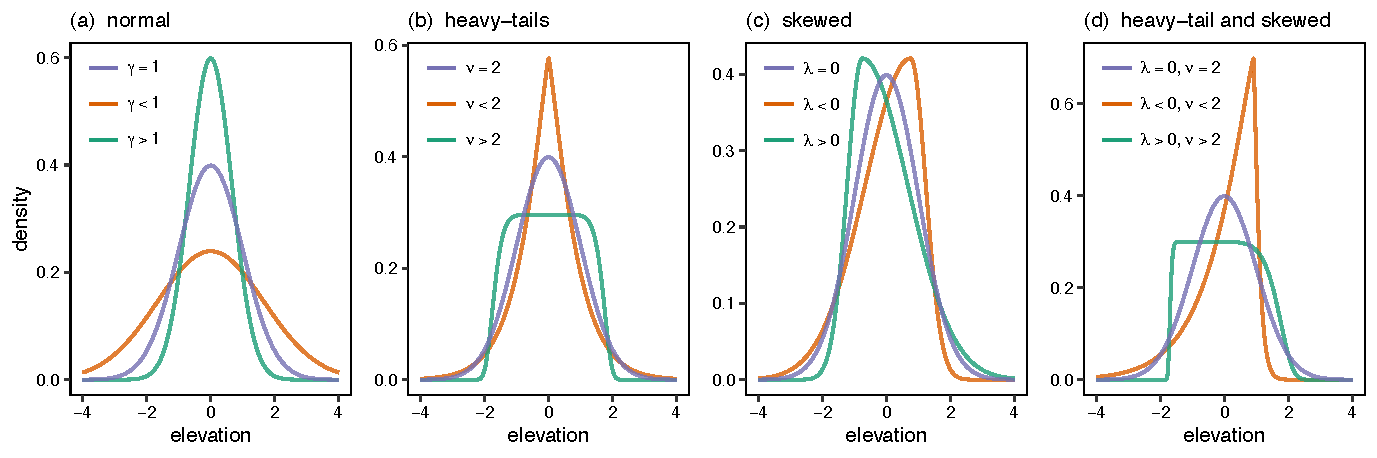
\includegraphics[width=1\textwidth]{figures/all-distributions}
	   \caption{Different response curves. Panel (a) shows the distribution shapes characterized by Eq.~(\ref{eq:baseline-response}) for different values of $\beta$, $\alpha$ and $\gamma$. Panel (b) shows the distribution shapes characterized by Eq.~(\ref{eq:generalized-response}) for different values of $\beta$, $\alpha$ and $\nu$, when $\gamma=1$. Panel (c) shows the distribution shapes characterized by Eq.~(\ref{eq:skewed-response}) for different values of $\beta$, $\alpha$ and $\lambda$, when $\gamma=1$. Panel (d) shows the distribution shapes characterized by Eq.~(\ref{eq:heavy-skewed-response}) for different values of $\beta$, $\alpha$, $\lambda$ and $\nu$, when $\gamma=1$. Notice that for all panels, we chose $\alpha$ values such that $\text{p}_i = \exp(-\alpha_i)$.
	   }
      \label{fig:response}
\end{figure}

\subsubsection*{Model priors}
The model structure described above allows us to explicitly incorporate all prior knowledge that we have regarding species' distributions contained in the floristic database. To do so, we define the prior distributions for the parameters in model (\ref{eq:baseline-response}) as:
\begin{equation} 
\begin{split}
\beta_{i}  & \sim \text{MVNormal}\left(\hat{\beta}, \Sigma^{\beta}\right)\\
\text{log}(\gamma_{i})  & \sim \text{MVNormal}\left(\hat{\gamma}, \Sigma^{\gamma}\right)\\
\text{log}(\alpha_{i}) & \sim \text{Normal}\left(\hat{\alpha}, \sigma_{\alpha}\right)\\
\hat{\beta}, 
\hat{\gamma}, 
\hat{\alpha}  & \sim \text{Normal}\left(0,1\right)\\
\sigma_{\alpha}  & \sim \text{Exponential}\left(1\right)
\end{split}
\label{eq:baseline-priors}
\end{equation} 
where parameters $\gamma_i$ and $\beta_i$ are expressed as multivariate normal distributions---i.e.~Gaussian processes---such that $\Sigma^{\beta}$ and $\Sigma^{\gamma}$ are variance-covariance matrices describing species' similarity in terms of their average climatic suitability and range of variation along the different environmental gradients, respectively. We define these variance-covariance matrices as follows:
\begin{equation} 
\Sigma_{ij} = \eta\,\text{exp}\left(-\rho {D_{ij}}^2\right) + \delta_{ij} \sigma ,
\label{eq:covariance-baseline}
\end{equation}
where $\Sigma_{ij}$ characterizes the covariance between any pair of species $i$ and $j$, and $\delta_{ij}$ is the Kronecker delta. Such a covariance structure declines exponentially with the square of a distance matrix $D_{ij}$, which characterize differences between species computed using our prior information. In the floristic database, this information is represented by the set of ordinal traits specified for the different species. While there are many different ways to turn ordinal data into distance matrices, we choose to use a mixed-membership stochastic block model because it allows us to deal with cases of missing data (see Supplementary Methods for extended details; \citealt{godoy-loriteAccurateScalableSocial2016}). In each covariance matrix, the hyperparameter $\rho$ determines the rate of decline of the covariance between any two species, and $\eta$ defines its maximum value. The hyperparameter $\sigma$ describes the additional covariance between the different observations for any given species. For all these hyperparameters, we choose weakly informative priors such that $\sigma , \eta \sim \text{Exponential}\left(1\right)$ and $\rho\sim \text{Exponential}\left(0.5\right)$. Notice that other structures can be used to define the covariance matrices of the different Gaussian processes \citep{mcelreathStatisticalRethinkingBayesian2020}, including structures that account for multiple distance matrix $D_{ij}$ for any given parameter.

\subsubsection*{Sampling the posterior}
We generated the posterior samples for the Bayesian models with the Hamiltonian Monte Carlo algorithm implementation provided by the R packages `rstan' and `cmdstanr' \citep{standevelopentteamRStanInterfaceStan2021}. Sampling models like the ones described above can be computationally very intensive. This is especially true when using ordered categorical likelihood functions (see \citealt{standevelopmentteamStanModelingLanguage2021}). Therefore, we focus on those species for which we have at least 20 occurrences when modelling both binary data and ordinal data.

To test the performance of the model as well as our choice of prior distributions, we modelled simulated data and compared the sampled posterior distributions to the data-generating parameters (see Code Availability section). Notice that using the link function in Eq.~(\ref{eq:baseline-response}) could cause problems when sampling the model, and some adjustments need to be made when specifying the model (see Code Availability section). To perform the data analysis and generate the figures, we used some of the functions available with the R package `rethinking' \citep{mcelreathStatisticalRethinkingBayesian2020}.

\subsection*{Modifying the baseline model}
%We proposed a baseline model that is naive regarding how the data is distributed, and yet accounts for all prior information that we have about the system. Now, we want to modify this model to test the extent to which empirical species' distributions showcase different properties, while preserving both the interpretation of the parameter estimates and prior information. We focused on two properties: fat-tailed and skewed responses. 

%To modify our baseline model, we propose new species' response curves we follow three criteria: (i) the probability distribution must have a defined variance and mean, (ii) the Gaussian shape must be a special case of the probability distribution, and (iii) there must be a re-parametrization of the model that allows us to keep the same prior information and interpretable parameters.

We proposed a baseline model that is naive regarding how the data is distributed, and yet accounts for all prior information that we have about the system. Now, we want to modify this model to test the extent to which empirical species' distributions showcase different shapes. We focused on two properties: fat-tailed and skewed responses. While there are several model structures that could account for these properties, we propose new species' response curves following three criteria. First, the probability distribution of a species along an environmental gradient must have a defined mean and variance. This is important because we know that species naturally have different environmental preferences as well as finite geographic ranges. Second, the Gaussian shape must be a special case of the probability distribution, allowing species to showcase variation regarding the presence (or lack thereof) of any given pattern. Finally, there must be a re-parametrization of the model that allows us to keep the same prior information and interpretable parameters.

\subsubsection*{Fat-tailed response curve}
Fat-tailed distributions represent distributions with relatively high representation of extreme events. While many different distributions exhibit this property, we decided to accommodate this feature into our baseline model by considering a response curve that follows a generalized error distribution. Such a distribution is useful because the Gaussian shape is a special case of it, and it contains a parameter that regulates the level of kurtosis---ranging from longer to shorter tails than the Gaussian case (Fig~\ref{fig:response}b). In particular, we can adapt Eq.~(\ref{eq:baseline-response}) to present this non-linear form as follows:
\begin{equation}
\begin{split}
\text{log}\left(p_{ij}\right) = -\alpha_{i} - \gamma^{\prime}_{i}\, |x_{j}-\beta_{i}|^{\nu_{i}} ,
\end{split}
\label{eq:generalized-response}
\end{equation}
where $\gamma^{\prime}_{i} = g(\gamma_{i}, \nu_{i})$, and $\nu_{i}$ is a parameter that describes the kurtosis of the distribution, which we define as $\nu_{i}\in\left(1, \infty\right)$. Following this, we choose an adaptive prior for this set of new parameter such that $\log\left(\nu_{i}-1\right)\sim \text{Normal}\left(\hat{\nu}, \sigma_{\nu}\right)$, where $\hat{\nu}\sim\text{Normal}\left(0, 1\right)$ and $\sigma_{\nu}\sim\text{Exponential}\left(2\right)$. Given the relationship between $\gamma^{\prime}_{i}$ and $\gamma_{i}$,  we can re-parametrize the model and follow Eq.~(\ref{eq:baseline-priors}) to define the prior distributions (see Supplementary Table 2; \citealt{nadarajahGeneralizedNormalDistribution2005}). Notice that the Gaussian distribution will naturally emerge when $\nu_i=2$.

Alternatively, we could have used other distributions that present fat tails and fulfil the selection criteria described above. For example, the non-standardized Student's t-distributions is an interesting distribution because, as opposed to the generalized error distribution, it allows for fat tails without generating a cusp at the center (see Fig~\ref{fig:response}b). However, we avoided using the non-standardized Student's t-distributions because it does not allow for tails that are lighter than normal (e.g.~$\nu_i>2$ in Eq.~\ref{eq:generalized-response}; Fig~\ref{fig:response}b), and the sampling of the model can be somewhat more challenging (ref). 

\subsubsection*{Skewed response curve}
Skewed responses present steeper declines towards either side of the distribution. One way to accommodate this feature in our models is by considering a skewed normal distribution. As for the case described above, the Gaussian is a special case of this distribution, and it contains a parameter that controls for the level and direction of `skewness' (Fig~\ref{fig:response}c). Importantly, this distribution presents normal-like tails; therefore, the added skewness does not make additional assumptions regarding how species are distributed along the gradient. To test for the existence of this feature, we modified Eq.~(\ref{eq:baseline-response}) as
\begin{equation}	
\begin{split}
\text{log}\left(p_{ij}\right) = -\alpha_{i} - \gamma^{\prime}_{i}\left(\frac{x_{j}-\beta^{\prime}_{i}}{1+\lambda_{i}\,\text{sgn}\left(x_{j}-\beta^{\prime}_{i}\right)}\right)^{2} ,
\end{split}
\label{eq:skewed-response}
\end{equation}
where $\gamma^{\prime}_{i} = q_{1}\left(\gamma_{i}, \lambda_{i}\right)$, $\beta^{\prime}_{i} = q_{2}\left(\gamma_{i}, \beta_{i}, \lambda_{i}\right)$, and $\lambda_{i}$ is a parameter that describes the skewness of the distribution such that $\lambda_{i}\in\left(-1, 1\right)$. The function $\text{sgn}\left(x\right)$ characterizes the sign function.  We chose $\lambda_i$ to have an adaptive prior such that $\text{logit}\left(\frac{\lambda_{i}+1}{2}\right)\sim \text{Normal}\left(\hat{\lambda}, \sigma_{\lambda}\right)$, where $\hat{\lambda}\sim\text{Normal}\left(0, 1\right)$ and $\sigma_{\lambda}\sim\text{Exponential}\left(1\right)$. Notice that this model can be re-parametrized following $q_1$ and $q_2$, allowing us to set the rest of the prior distributions as described for the baseline model (see Supplementary Table 2; Code Availability section). In this case, the Gaussian distribution is a special case of Eq.~(\ref{eq:skewed-response}) when $\lambda_{i}=0$ \citep{ashourApproximateSkewNormal2010}.

\subsubsection*{Fat-tailed and skewed response curve}
Finally, one could consider a response curve with both kurtosis and skewness. A convenient way to achieve this is by using a response curve that follows a skewed generalized error distribution. This is a combination of the two distributions described above, containing two parameters that control for both the level and direction of kurtosis and skewness (Fig~\ref{fig:response}d). The skewed generalized error distribution can be considered by modifying the species' response curve in Eq.~(\ref{eq:baseline-response}) as
\begin{equation}	
\begin{split}
\text{log}\left(p_{ij}\right) = -\alpha_{i} - \left(\frac{\gamma^{\prime}_{i}\,|x_{j}-\beta^{\prime}_{i}|}{1+\lambda_{i}\,\text{sgn}\left(x_{j}-\beta^{\prime}_{i}\right)}\right)^{\nu_{i}} ,
\end{split}
\label{eq:heavy-skewed-response}
\end{equation}
where $\gamma^{\prime}_{i} = f_{1}\left(\gamma_{i}, \nu_{i}, \lambda_{i}\right)$, $\beta^{\prime}_{i} = f_{2}\left(\gamma_{i}, \beta_{i}, \nu_{i}, \lambda_{i}\right)$, and $\nu_{i}$ and $\lambda_i$ are parameters that control the kurtosis and skewness of the distribution, respectively. We define $\nu_i$, $\lambda_i$ and their prior distributions as in Eq.~\ref{eq:generalized-response} and \ref{eq:skewed-response}, respectively. Again, we can re-parametrize the model following $f_1$ and $f_2$, and set the rest of the prior distributions as in the baseline model (see Supplementary Table 2; Code Availability section). Notice that the generalized error distribution (Eq.~\ref{eq:generalized-response}) and the skew normal distribution (Eq.~\ref{eq:skewed-response}) are special cases of Eq.~(\ref{eq:heavy-skewed-response}) when $\lambda_i=0$ and $\nu_i=2$, respectively.

%One way to test the extent to which species' physiological traits inform the kurtosis or skewness of the distribution of any species $i$ is by characterizing $\nu_{i}$ or $\lambda_{i}$ as Gaussian processes. That is, we can consider the prior distribution for these parameters as multivariate normal with a variance covariance matrix $\Sigma$. As described before, this variance-covariance matrix can be estimated following Eq.~(\ref{eq:covariance-baseline}), and its structure can shed light on how informative the physiological traits are. Likewise, we could instead use Eq.~(\ref{eq:covariance-complex}) and test the effectiveness of other prior information in explaining the skewness of species' distributions.

\subsection*{Evaluating the log-likelihood}
One way to understand the shape of distributions is by evaluating the computed log-likelihood values across the environmental gradient. Comparing these values, one can understand what aspects of the shape of distributions are missing. To do so, for every sample of the model, we computed the log-likelihood values and the normalized probability distribution. This normalized probability is defined such that its maximum is set to 1 for all species in our dataset. In particular, for a heavy-tailed and skewed response, the normalized probability distribution was calculated for every sample of the Bayesian model using Eq.~(\ref{eq:heavy-skewed-response}), where $\alpha_i$ was set to 0 for any value of $x_{j}$. Notice that the normalized probability distribution is interesting when comparing the log-likelihood values across species because it can be used to understand whether the model errors are at the tails of the distributions or their center. 

\section*{Results}
We studied the distribution data to characterize species' realized niches along the main axis of variation of all environmental variables. Using the presence and absence of species across sites as the response variable, we sampled the posterior distributions of the baseline model, accounting for the information in the floristic database regarding species' indicator values and range of variation. This allowed us to map the center and variance of species' distributions along the environmental gradient (Fig.~\ref{fig:correlation}).  Studying the relationship between these properties, we found these to be negatively correlated (i.e.~$\beta_{i}$ and $\gamma_{i}$ in the baseline model were positively correlated; Fig.~\ref{fig:correlation}). This means that species found at lower elevations have generally wider distributions than those at higher elevations. The same relationship was found when using instead elevation or mean temperature as explanatory variables (Supplementary Fig.~XX) as well as when using ordinal data (Supplementary Fig.~XX); however, the pattern was not present along the second main axis of variation of our environmental variables (Supplementary Fig.~XX). The comparison between the other parameter estimates revealed additional, somewhat more expected, relationships. In particular, we found the amplitude of distributions to be positively and negatively correlated with their mean and variance, respectively (i.e. $\alpha_{i}$ is positively correlated with $\beta_{i}$ and $\gamma_{i}$; Supplementary Fig.~XX). This implies that, at higher elevations, species' distributions generally have lower amplitudes.

\begin{figure}[h]
  \centering
    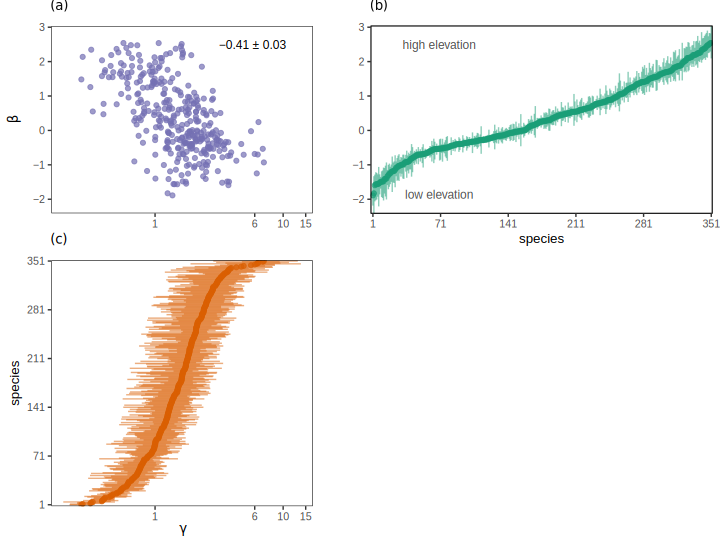
\includegraphics[width=0.9\textwidth]{figures/figure1-prime}
    	  \vspace{0.1cm}
	   \caption{Relationship between the posterior distributions for parameters $\beta_i$ and $\gamma_i$ from Eq.~(\ref{eq:baseline-response}) across species. Panel (a) describes the relationship between the mean ($\beta_i$) and variance ($\propto\gamma_i^{-1}$) of distributions. Every dot characterizes the average value of the corresponding posterior distributions for any given species. The value in the bottom-left corner of the plot displays the Pearson's correlation coefficient between the parameters calculated across all samples. Panel (b) displays the estimates for the center of species' distributions along the environmental gradient. Panel (c) displays the estimates for the variance of species' distributions along the environmental gradient. In (b) and (c), the points represent the mean of the posterior distributions, and the corresponding lines characterize the 89\% confidence intervals.}
	   %7.5-5.5
      \label{fig:correlation}
\end{figure}

Maintaining the symmetry of species' distributions, we then allowed the kurtosis---or shape of the tails---of these to vary in different ways. To do so, we changed the response curve of our Bayesian model to follow a generalized error distribution (Eq.~\ref{eq:generalized-response}). A comparison of the WAIC values showed this non-linear regression to outperform the baseline model (Supplementary Fig.~XX). Studying the resulting posterior distributions, we found the average kurtosis of the distributions to be slightly greater than zero, which corresponds to distributions with longer tails than the Gaussian case (Fig.~\ref{fig:kurtosis-skewness}). However, the parameter controlling for the kurtosis $\nu_i$ displayed a lot of variation across species (Supplementary Fig.~XX), which might indicate that the shape of the tails is species-specific. 

\begin{figure}[ht]
  \centering
    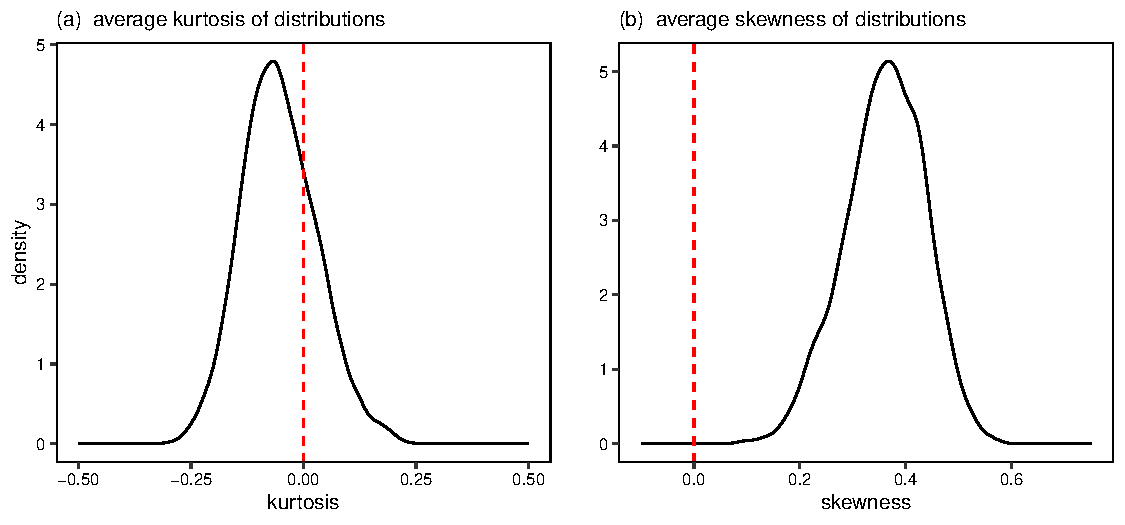
\includegraphics[width=0.9\textwidth]{figures/kurto-skew}
    	  \vspace{0.1cm}
	   \caption{Average kurtosis and skewness of species' distributions. Calculated using the posterior distributions of parameters $\hat{\nu}$ and $\hat{\lambda}$ from the models (see Supplementary Table XX), the two panels describe the average (a) kurtosis and (b) skewness of distributions. Panel (a) displays the results obtained using response curves that follow a generalized error distribution (black line) and a skewed generalized error distribution (yellow line). Panel (b) displays the results obtained using response curves that follow a skewed normal distribution (black line) and a skewed generalized error distribution (yellow line). In both cases, the gray dotted line indicates the conditions by which species are normally distributed along the environmental axis.}
      \label{fig:kurtosis-skewness}
      %7.5-3
\end{figure}

Using Eq.~(\ref{eq:skewed-response}), we next studied the skewness of species' distributions. Based on the estimates for the WAIC values, this model outperformed the first two (Supplementary Fig.~XX), which sheds light on the naturally skewed nature of species' distributions. Perhaps most importantly, studying the mean value of the skewness across species, we found this to be consistently below zero (Fig.~\ref{fig:kurtosis-skewness}). This indicates that species' distributions generally present steeper declines towards higher elevations (i.e. $\hat{\lambda}<0$; Fig.~\ref{fig:response}). The same was true when using a model that allowed for both fat-tailed and skewed response curves (Eq.~\ref{eq:heavy-skewed-response}). This model outperformed the rest, presenting Akaike weights close to 1 (Supplementary Fig.~XX), suggesting that both the kurtosis and skewness are useful properties to describe empirical distributions (Fig.~\ref{fig:kurtosis-skewness}). A study of how the prior knowledge we had regarding species' environmental preferences, range of variation and ecological strategies informed the different parameters of the model is presented in the Supplementary Note XX. %Comparing the prior and posterior distributions for the hyperparameters in the. 

The model characterizing fat-tailed and skewed distributions allowed us to study the posterior distributions for the parameters describing the mean, variance, amplitude, kurtosis and skewness of species realized niches altogether. We observed that different types of species seem to present characteristically different distributions (Fig.~\ref{fig:pairwise}). Focussing on the negative correlation between the mean and variance of species' distributions, we found some species to escape some of the aforementioned macroecological constraints (Supplementary Fig.~XX).  Moreover, recent and historical range expanders are often found at lower altitudes, presenting higher amplitudes and distributions that appear to showcase steeper declines towards lower elevations. Notice the nature of these results does not depend on the presence or absence of a species at the edge of the sampling area, as the same model produced comparable results when using simulated and bootstrapped data (Supplementary Note XX and Supplementary Fig.~XX). Moreover, these results did not substantially change when using ordinal data (Supplementary Fig.~XX).

%The comparison across other types of species also provided us with additional interesting mappings. For example,... Likewise, other pairwise comparisons across parameters also revealed additional macroecological constrains (Supplementary Fig.~XX).

%The same was not true when clustering species based on their changes in abundance over the years (Fig.~XX). 
%, and it does not seem to depend on species' type or reflect species' abundance change tendency over the years (Fig.~\ref{fig:universality}). T
%Moreover, species' physiology seems to strongly shape this parameter, which suggest that distribution skewness is an intrinsic property of species (New Fig.~XX).

\begin{figure}[ht]
  \centering
    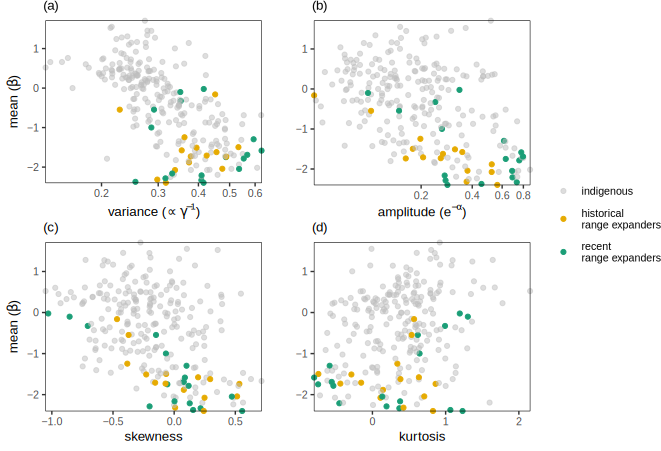
\includegraphics[width=0.9\textwidth]{figures/figure3}
    	  \vspace{0.1cm}
	   \caption{Comparing the distributions of different types of species. Focussing on the differences between indigenous, historical range expanding and recent range expanding species, the panels describe the relationship between the basic properties of their distributions. Panels (a-d) characterize the relationship between the mean, and the variance, amplitude, skewness and kurtosis of the species' distributions (Supplementary Table XX). The points in every panel are calculated as the average value across all samples of the model. %The analogous results found for species classified accroding to their population change tendency over the years is presented in Supplementary Fig~XX. The ellipses characterize the 1 standard deviation ellipses for each species type. 
	   }
	   %7-4.5
      \label{fig:pairwise}
\end{figure}

Finally, we wanted to identify what aspects of the shape of distributions we were still missing. We used the computed log-likelihood values and normalized probabilities to understand where our best performing model fails to capture the variation in empirical plant distributions. We found most data points to be located at the tails of distributions ($\text{normalized probability}\,\approx\,0$) and to present high log-likelihood values (Supplementary Fig.~XX). This is not surprising as the study area spans an extensive altitude gradient, and species' distributions are generally narrow relative to it; therefore, the model accurately predicts that species are usually absent in those sampling sites that fall relatively far from the center of their distributions. However, studying instead only those points for which the model did not perform well (with a $\text{likelihood}\leq 0.5$), we found these to generally be associated with high normalized probabilities (Fig.~\ref{fig:loglik}). This indicates that the unexplained variation is often found at the center of species' distributions. Similar results were found when using ordinal data (Supplementary Fig.~XX).

\begin{figure}[ht]
  \centering
    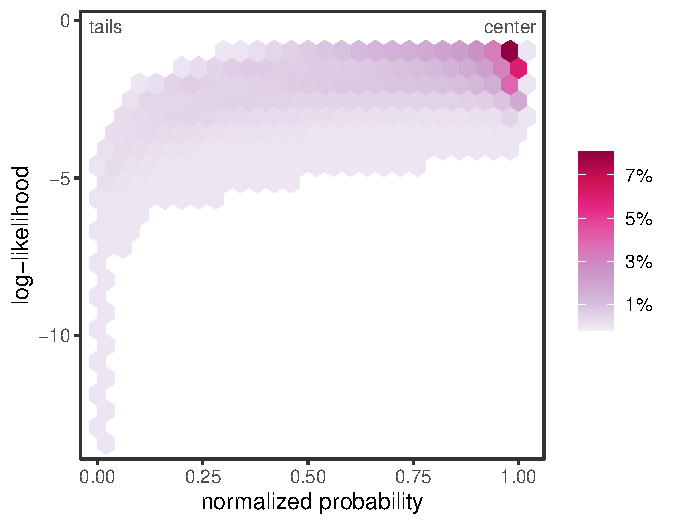
\includegraphics[width=0.5\textwidth]{figures/loglik-notshow-bin}
    	  \vspace{0.1cm}
	   \caption{Studying the distribution of log-likelihood values. The graph maps the log-likelihood and normalized probability values for all species across all samples. Notice that in this figure there are only displayed those points that present a likelihood smaller than $0.5$. The mapping of all log-likelihood values is presented in Supplementary Fig.~XX.}
	   %5-4
      \label{fig:loglik}
\end{figure}

%The posterior distributions of the hyperparameters in Eq.~(\ref{eq:covariance-baseline}) revealed the value of this prior information on the different parameter estimates.  to understand the value of our prior information. 


%We then studied the level of information contained in physiological traits to explain the properties of distributions. Specifically, using Eq.~(\ref{eq:covariance-complex}), we accounted for both physiological and environmental traits in the variance-covariance structure for the mean and standard deviation of distributions. We information 
%As expected, the posterior distributions also showcase a positive relationship between... This is expected as ... Likewise, studying ... Following this, we added additional ... using Eq.~(\ref{eq:covariance-complex}). When studying plant... 
%Other interesting comparisons... The value of adding plant physiology as prior information for both the mean and standard deviation of the distributions. Informative in both case, specially for... Capturing some of bla bla bla.

%Then, we stud the tails of distributions by modifying the baseline model to account for different properties. Kurtois. Studying the parameter... Similar values were found for binary data and the model did not outperform the baseline model

% Next we studied the skewness of distributions, outpreforming the other models. When studying the parameter, we found that the mean skewness of species' distributions declined... Hypothesis! When accounting for plant physiology as priors for the skewness of distribution, we found this to be ... Figure and Hypothesis. The model also showcased the Rapopor's hypothesis...

%%%%%%%%%%%%%%%%%%%%%%%%%%%%%%%%%%%%%%%%%%%%%%%%%%%%%%
%%       DISCUSSION
%%%%%%%%%%%%%%%%%%%%%%%%%%%%%%%%%%%%%%%%%%%%%%%%%%%%%%
\section*{Discussion}
In this work, we used non-linear response curves to model the distribution of species across an environmental gradient. First, we used a baseline model that considered these as bell-shaped, and we studied the relationship between the basic parameters characterizing them. We found both the amplitude and variance of distributions to be negatively correlated with elevation. Considering more complex response curves, we then found species' distributions to also present non-normal tails and skewed shapes. Specifically, we found species' distributions to generally be characterized by fat tails and steeper declines towards higher elevations. That said, the nature of these distributions was not homogeneous across species, as some of them presented singularly different properties. This is the case of rapid and historical range expanders, often found in warmer environments, with distributions presenting higher amplitudes and skewed responses towards high altitudes. Finally, we studied the variation that remained unexplained by the best performing model. We found this unexplained variation to be generally located at the center of distributions, which identified potential general properties of empirical distributions that were missed by our model. Putting this all together, our results uncovered several aspects of the shape of empirical plant distributions and revealed crucial differences between the way species are assembled along environmental gradients. 

Our approach allowed us to parsimoniously compare the shape of the species' realized niches along an altitude gradient, testing for the existence of several macroecological patterns. For example, the Rapoport's rule predicts wider ranges of species at higher latitudes and altitudes \citep{stevensElevationalGradientAltitudinal1992}; and therefore, one might expect a positive correlation between the mean and variance of species distributions. A common explanation for the Rapoport's rule is that climatic variability selects for species with greater climatic tolerances. But while this pattern has been largely studied for multiple systems and across gradients \citep{mccainElevationalRapoportRule2013}, contrasting evidence suggests that this rule is not pervasive across species \citep{ribasRapoportEffectWidespread2006, bhattaraiCanRapoportRule2006, mccainElevationalRapoportRule2013}. Our results seem to contradict the predictions of the Rapoport's rule, as we observed a negative correlation between species' range and elevation. Moreover, other properties of species' distributions---such as their amplitude---were also significantly correlated with species' ranges. This is interesting because it hints at the existence of some general macroecological constraints that dictate the way different species assemble across environments. That said, our results also suggest that species such as neophytes and archeophytes might not obey this same constraints, as these were singularly positioned along the gradient (Supplementary Fig.~XX). 

The level of skewness of species' distribution as well as the variability in the shape of theirs tails diverged from traditionally assumed bell-shaped curves. This allowed us to focus on other interesting macroecological hypotheses. For instance, the so-called abiotic stress limitation hypothesis predicts species' distributions to present steeper declines towards stressful conditions \citep{austinCommunityTheoryCompetition1990}. \citet{normandImportanceAbioticStress2009} tested this for vegetation data using \citeauthor{huismanHierarchicalSetModels1993}'s statistical models for several independent species, finding no clear support for such a hypothesis (but see \citealt{ziffer-bergerSpatialPatternsProvide2014}). Our results, however, showcased species' distributions to generally present steeper declines towards higher elevations, providing clear evidence of this geographical pattern. Moreover, we were able to highlight the degree to which different species might present different levels of decline towards stressful conditions, as plants found at low elevations---such as recent and historical range expanding species---displayed contrasting levels of skewness. This is important because it could provide glimpses of the different stages of species' assembly processes, with range expanders' distributions trending towards higher elevations. 

There are many other properties characterizing empirical distributions that might not have been captured by the different models. One possible way to untangle these properties is by studying the unexplained variation in the empirical data. We observed that this variation is often located at the center of distributions, which suggests that the aspects of their shape not picked up by the models involve those points at the peak of the distributions. This observation is directly linked to another macroecological pattern: the so called abundant-center hypothesis \citep{sagarinAbundantCentreDistribution2002}. This hypothesis predicts species to be most abundant at the center of their distributions, and it is an implicit assumption at the core of most modelling approaches. Namely, if one is only willing to assume that species have finite geographic ranges, the abundant-center hypothesis is a consequence our state of ignorance (i.e.~the maximum entropy distribution). That said, several studies have pointed out that the abundant-center hypothesis is not pervasive in empirical distributions \citep{wagnerSimilarPerformanceCentral2011, pirononGeographicVariationGenetic2017, dallasSpeciesAreNot2017}, suggesting that population abundance could often be more strongly driven by interactions and community structure than the environment \citep{dallasSpeciesAreNot2017}. Our results, for both binary and ordinal data, support these observations, suggesting that the species' probability of appearance---as well as likelihood of presenting high abundance at a given site---might not ubiquitously be highest at the center of their distributions. Allowing species to showcase other distribution shapes, such as those including multimodal or plateau peaks, could potentially resolve some of the unexplained variation. Indeed, studying the tails of species' distributions, we observed several species presenting low kurtosis levels. While this implied that these distributions had shorter tails than normal, it also reflected plateau-shaped response curves (e.g.~$\nu>2$ in Fig.~\ref{fig:response}b).

The different hypotheses regarding the shape of species' distributions address central topics in ecology and evolution \citep{sagarinAbundantCentreDistribution2002}. These distributions are the result of environmental variability \citep{helmuthClimateChangeLatitudinal2002, butterfieldEnvironmentalFilteringIncreases2015}, biotic interactions \citep{hastingsUnexpectedSpatialPatterns1997} and historical contingencies \citep{frickEmergingDiseaseCauses2010}, and their shape determines gene flow \citep{haldaneRelationDensityRegulation1956, lesicaWhenArePeripheral1995, pirononGeographicVariationGenetic2017} and energy balances along gradients \citep{hallDistributionAbundanceOrganisms1992}. Perhaps most importantly, the shape of species' distributions will influence their responses to environmental changes \citep{channellDynamicBiogeographyConservation2000}, and it could therefore be used as an ecological compass to inform conservation and management decisions \citep{channellTrajectoriesExtinctionSpatial2000}. In this context, we identify two areas we feel represent key steps from which to move forward. First, trait data could crucially inform the different parameters controlling the shape of distributions. For example, if the skewness of species' distributions is the result of uneven environmental tolerances along the gradient \citep{sundayGlobalAnalysisThermal2011}, this information should be accounted for analogously to the way we used the expert knowledge on plants' environmental preferences. The same is true for species' ecological strategies, with aspects regarding their competitive ability potentially informing the shape of distributions. Second, from a performance standpoint, the models presented here will likely do a worse job at predicting species' occurrences than some of the distribution models developed over the recent years \citep{norbergComprehensiveEvaluationPredictive2019}, including those accounting for spatial autocorrelation \citep{ovaskainenUncoveringHiddenSpatial2016}, associations between species \citep{tikhonovJointSpeciesDistribution2020}, and some non-parametric approximations \citep{harrisGeneratingRealisticAssemblages2015}. However, our models have clear interpretable parameters, and can be used to directly compare the shape of species' realized niches. These comparisons could be used to generate hypotheses regarding where and when different species might strongly interact with one another along an environmental gradient \citep{louthanWhereWhenSpecies2015}, making ecologically-informed predictions regarding the presence and absence of these relationships \citep{SIASH}.


%A consequence of Ecological interactions (Hochberg Ives 1998), energy balances along gradients (Hall Standford Hauer 1992), 
% From article: These hypotheses directly address many fundamental issues in ecology and evolution, such as how genes flow between populations, as well as applied ecological issues, such as how populations will respond to climate change and what populations should be the focus oflimited conservation resources. If species are mostabundant at the edge of their range, genes and individuals may flow from the edges to the centre, leading to the opposite conclusions of abundant centre-based hypotheses. Alternatively, if species were most abundant at only one edge of the range (e.g. species became gradually more abundant toward the south edge of the range), the direction and magnitude of gene swamping or population outbreaks could not be predicted without identifying specific study locations. \citep{sagarinAbundantCentreDistribution2002}.
% From article: The abundant centre distribution, if present, also simplifes many hypo-theses about population dynamics, conservation biology,and factors that set species' ranges \citep{sagarinAbundantCentreDistribution2002}.
% From article: This theoretical work relates to some of the most fundamental and practical issues in ecology, including questions of where to situate nature reserves, where pest outbreaks are expected, how species will respond to climate change, and the genetic structure of population \citep{sagarinAbundantCentreDistribution2002}.
%From article: Understanding how interspeci-fic interactions, natural enemies, environmental forces anddispersal barriers influence the existence of distance–abundancerelationship remains an open question; one, when answered,may provide an underlying basis for the emergence of themacroecological pattern \citep{dallasSpeciesAreNot2017}

%Understanding the extend to which this new properties are across species could potentially

%Refs for center-abundance hypo: Hengeveld & Haeck1982; Brown 1984; Holt et al. 1997; McGill & Collins 2003)

%From article: species interactions andcommunity structure may be more important in regulatingpopulation abundance than the environment Second, the spa-tial distribution of abundance, and subsequent distance–abun-dance relationships, may be limited by dispersal boundaries orunmeasured ecological interactions. For instance, coasts andmountain ranges represent obvious barriers to species spread.Species abundance may be highest at the barrier (Brown et al.1996), with the putative explanation being directional disper-sal against a barrier, and an environment capable of sustain-ing relatively high species abundance. \citep{dallasSpeciesAreNot2017}
% From article: tandem action of niche and dispersal processes appears to play an important role in constraining this species’ northern latitudinal range \citep{baerDecliningDemographicPerformance2019}.

%Finally, we identify three areas we feel represent key steps from which to move forward. First,... Is species' physiology informative to explain the pattern? Further test of the ability of traits to predict those parameter estimates. Second,... Using this information to understand where jSDMs estimate interactions between species. Third,... understanding the dynamical implications of certain properties...

\clearpage
\bibliography{references2}

\end{document}
